\def\raggedright{}
\documentclass[final,hyperref={pdfpagelabels=false}]{beamer}
%\usepackage{grffile}
%\mode<presentation>{\usetheme{I6dv}}
\usepackage[french]{babel}
\usepackage[utf8]{inputenc}
\usepackage[T1]{fontenc}
\usepackage{ae,aecompl}
\usepackage{amsmath,amsthm, amssymb, latexsym}
%\usepackage{figlatex}
\usepackage{multicol}
\usepackage{tikz,url}
\usetikzlibrary{shapes.geometric}
%\usepackage{times}\usefonttheme{professionalfonts}  % obsolete
%\usefonttheme[onlymath]{serif}
\boldmath
%\usepackage[orientation=portrait,size=custom,height=20cm,width=20cm,debug]{beamerposter}
%\usepackage[orientation=portrait,size=custom,debug]{beamerposter}
% change list indention level
% \setdefaultleftmargin{3em}{}{}{}{}{}
\definecolor{orange1}{rgb}{0.988,0.686,0.243}
\definecolor{orange2}{rgb}{0.961,0.475,0.000}
\definecolor{orange3}{rgb}{0.808,0.361,0.000}

% Work around a bug in beamer?
% http://tex.stackexchange.com/questions/4436/beamer-undefined-control-sequence
\providecommand\thispdfpagelabel[1]{}

\setlength{\paperwidth}{20cm}
\setlength{\paperheight}{20cm}
\setlength{\textwidth}{18cm}
\setlength{\textheight}{18cm}
\edef\fontscale{0.5}    % fontscale=(1/sqrt(2))^3

%%%%%%%%%%%%%%%%%%%%%%%%%%%%%%%%%%%%%%%%%%%%%%%
%%%%%%%%%%%%%%%%%%%%%%%%%%%%%%%%%%%%%%%%%%%%%%%
%%%%%%%%%%%%%%%%%%%%%%%%%%%%%%%%%%%%%%%%%%%%%%%
%%%%%%%%%%%%%%%%%%%%%%%%%%%%%%%%%%%%%%%%%%%%%%%
\usepackage{fp}
\edef\myfontscale{1.0}
%% normalize scale depending on poster size
\FPupn{\myfontscale}{myfontscale fontscale * 2 round}
%% scalable vector fonts
\edef\fontSizeX{12}\edef\fontSizeY{14}
\FPupn{\resulttinyX}{myfontscale fontSizeX * 2 round}
\FPupn{\resulttinyY}{myfontscale fontSizeY * 2 round}
\renewcommand*{\tiny}{\fontsize{\resulttinyX}{\resulttinyY}\selectfont}

\edef\fontSizeX{14.4}\edef\fontSizeY{18}   
\FPupn{\resultscriptsizeX}{myfontscale fontSizeX * 2 round}
\FPupn{\resultscriptsizeY}{myfontscale fontSizeY * 2 round}
\renewcommand*{\scriptsize}{\fontsize{\resultscriptsizeX}{\resultscriptsizeY}\selectfont}

\edef\fontSizeX{17.28}\edef\fontSizeY{22}
\FPupn{\resultfootnotesizeX}{myfontscale fontSizeX * 2 round}
\FPupn{\resultfootnotesizeY}{myfontscale fontSizeY * 2 round}
\renewcommand*{\footnotesize}{\fontsize{\resultfootnotesizeX}{\resultfootnotesizeY}\selectfont}

\edef\fontSizeX{20.74}\edef\fontSizeY{25}
\FPupn{\resultsmallX}{myfontscale fontSizeX * 2 round}
\FPupn{\resultsmallY}{myfontscale fontSizeY * 2 round}
\renewcommand*{\small}{\fontsize{\resultsmallX}{\resultsmallY}\selectfont}

\edef\fontSizeX{24.88}\edef\fontSizeY{30}
\FPupn{\resultnormalsizeX}{myfontscale fontSizeX * 2 round}
\FPupn{\resultnormalsizeY}{myfontscale fontSizeY * 2 round}
\renewcommand*{\normalsize}{\fontsize{\resultnormalsizeX}{\resultnormalsizeY}\selectfont}

\edef\fontSizeX{29.86}\edef\fontSizeY{37}
\FPupn{\resultlargeX}{myfontscale fontSizeX * 2 round}
\FPupn{\resultlargeY}{myfontscale fontSizeY * 2 round}
\renewcommand*{\large}{\fontsize{\resultlargeX}{\resultlargeY}\selectfont}

\edef\fontSizeX{35.83}\edef\fontSizeY{45}
\FPupn{\resultLargeX}{myfontscale fontSizeX * 2 round}
\FPupn{\resultLargeY}{myfontscale fontSizeY * 2 round}
\renewcommand*{\Large}{\fontsize{\resultLargeX}{\resultLargeY}\selectfont}

\edef\fontSizeX{43}\edef\fontSizeY{54}
\FPupn{\resultLARGEX}{myfontscale fontSizeX * 2 round}
\FPupn{\resultLARGEY}{myfontscale fontSizeY * 2 round}
\renewcommand*{\LARGE}{\fontsize{\resultLARGEX}{\resultLARGEY}\selectfont}

\edef\fontSizeX{51.6}\edef\fontSizeY{64}
\FPupn{\resulthugeX}{myfontscale fontSizeX * 2 round}
\FPupn{\resulthugeY}{myfontscale fontSizeY * 2 round}
\renewcommand*{\huge}{\fontsize{\resulthugeX}{\resulthugeY}\selectfont}

\edef\fontSizeX{61.92}\edef\fontSizeY{77}
\FPupn{\resultHugeX}{myfontscale fontSizeX * 2 round}
\FPupn{\resultHugeY}{myfontscale fontSizeY * 2 round}
\renewcommand*{\Huge}{\fontsize{\resultHugeX}{\resultHugeY}\selectfont}

\edef\fontSizeX{74.3}\edef\fontSizeY{93}
\FPupn{\resultveryHugeX}{myfontscale fontSizeX * 2 round}
\FPupn{\resultveryHugeY}{myfontscale fontSizeY * 2 round}
\newcommand*{\veryHuge}{\fontsize{\resultveryHugeX}{\resultveryHugeY}\selectfont}

\edef\fontSizeX{89.16}\edef\fontSizeY{112}
\FPupn{\resultVeryHugeX}{myfontscale fontSizeX * 2 round}
\FPupn{\resultVeryHugeY}{myfontscale fontSizeY * 2 round}
\newcommand*{\VeryHuge}{\fontsize{\resultVeryHugeX}{\resultVeryHugeY}\selectfont}

\edef\fontSizeX{107}\edef\fontSizeY{134}
\FPupn{\resultVERYHugeX}{myfontscale fontSizeX * 2 round}
\FPupn{\resultVERYHugeY}{myfontscale fontSizeY * 2 round}
\newcommand*{\VERYHuge}{\fontsize{\resultVERYHugeX}{\resultVERYHugeY}\selectfont}

% set the normalfont (default)
\renewcommand*{\normalfont}{\normalsize}

%%%%%%%%%%%%%%%%%%%%%%%%%%%%%%%%%%%%%%%%%%%%%%%
%%%%%%%%%%%%%%%%%%%%%%%%%%%%%%%%%%%%%%%%%%%%%%%
%%%%%%%%%%%%%%%%%%%%%%%%%%%%%%%%%%%%%%%%%%%%%%%
%%%%%%%%%%%%%%%%%%%%%%%%%%%%%%%%%%%%%%%%%%%%%%%

%%%
%%% No navigation, thanks
%%%
\usenavigationsymbolstemplate{}

%\beamertemplategridbackground[1cm]

%\usepackage{snapshot} % will write a .dep file with all dependencies, allows for easy bundling

\usepackage{array,booktabs,tabularx}
\newcolumntype{Z}{>{\centering\arraybackslash}X} % centered tabularx columns
\newcommand{\pphantom}{\textcolor{ta3aluminium}} % phantom introduces a vertical space in p formatted table columns??!!

\listfiles

%%%%%%%%%%%%%%%%%%%%%%%%%%%%%%%%%%%%%%%%%%%%%%%%%%%%%%%%%%%%%%%%%%%%%%%%%%%%%%%%%%%%%%
\graphicspath{{figures/}}

\begin{document}
\begin{frame}{}

  \begin{center}
    \structure{\Huge CS IRL}

    \medskip
    \structure{\large Computer Science In Real Life}

    \bigskip
    \bigskip
    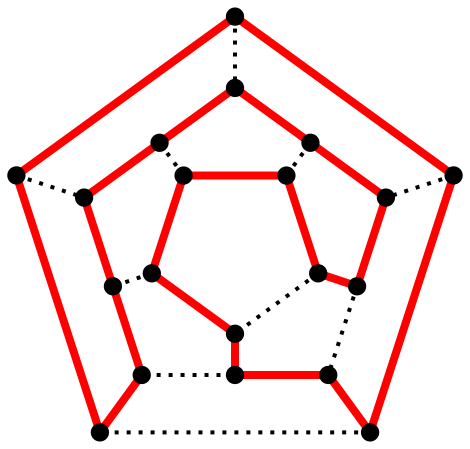
\includegraphics[width=.7\linewidth]{img/Hamiltonian_path.pdf}\label{img:hamiltonian}
  \end{center}
\end{frame}
%%%%%%%%%%%%%%%%%%%%%%%%%%%%%%%%%%%%%%%%%%%%%%%%%%%%%%%%%%%%%%%%%%%%%%%%%%%%%%%%%%%%%%%%
\begin{frame}
  \vspace{20\baselineskip}
  \vfill
  \begin{block}{À propos de ce document}
    \begin{itemize}
    \item \copyright\ 2011 membres du projet CS IRL. Tous droits réservés.

    \item CS IRL est un \alert{projet libre et ouvert}: vous pouvez copier et
      modifier librement les ressources de ce projet sous les conditions
      données par la CC-BY-SA (en bref, vous pouvez diffuser et modifier ces
      ressources à condition que vous donniez les mêmes droits aux utilisateurs
      de vos copies).
    \item La page web du projet est ici: \url{http://wiki.nybi.cc/index.php/CSIRL}
    \item Les sources des ressources du projet sont entre autres ici: \url{http://github.com/jcb/CSIRL}
    \item Si vous le souhaitez, vous pouvez nous joindre ici: \url{discussions@listes.nybi.cc}
    \end{itemize}
  \end{block}

  \begin{block}{\normalsize Crédits image}\footnotesize
    P\pageref{img:hamiltonian}: Chemin hamiltonien par Ch. Sommer,
    licence GFDL/CC-BY-SA
    \url{http://en.wikipedia.org/wiki/File:Hamiltonian_path.svg}

    P\pageref{img:matches}: Pyramide d'allumettes par M0tty, licence CC-BY-SA 
    \url{http://fr.wikipedia.org/wiki/Fichier:Pyramidal_matches.svg}
  \end{block}
\end{frame}
%%%%%%%%%%%%%%%%%%%%%%%%%%%%%%%%%%%%%%%%%%%%%%%%%%%%%%%%%%%%%%%%%%%%%%%%%%%%%%%%%%%%%%%%
\begin{frame}{Computer Science IRL -- Informatique sans ordinateur\\[-5pt]
  {\large Présentation du projet}}

% Contrairement à ce que beaucoup de monde pense, les ordinateurs ne sont pas la
% seule raison d'être de l'informatique. Pour preuve, ce projet développe
% diverses activités à faire avec des pions, des jetons ou des bouts de bois,
% mais sans aucun ordinateur et même sans électricité. Pourtant, ces petits jeux
% permettront à chacun de découvrir de manière ludique les notions au cœur de
% l'informatique: ce qu'est un algorithme et qu'est ce qui fait qu'un algorithme
% est meilleur qu'un autre, ou encore comment coder et transmettre une
% information.


  \begin{block}{CS IRL? Qu'est ce que c'est?}
    \begin{itemize}
    \item Des activités présentant les bases de l'informatique, mais sans
      ordinateur
    \item Pour chaque activité, un support matériel est proposé pour permettre
      d'\textit{apprendre avec les mains}
    \item Les activités sont rangées en séances cohérentes et progressives
%    \item C'est un projet libre, que vous pouvez télécharger, améliorer et
%      diffuser librement
    \item[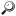
\includegraphics{img/rightpointing_magnifying_glass.pdf}]
      Computer Science In Real Life: Computer Science est la science
      informatique en anglais, tandis que IRL est l'abréviation utilisée sur
      internet pour décrire la vraie vie, ce qui n'est pas sur internet.
    \end{itemize}
  \end{block}

  \begin{block}{Les séances existantes dans la série}
    \begin{itemize}
    \item \structure{Séance 1:} Qu'est ce qu'un algorithme, et à quoi ça sert 
    \item \structure{Séance 2:} Comment les ordinateurs codent et manipulent les données (à
      venir)
    \item \structure{Séance 3:} Turzzle, le puzzle de programmation sans
      ordinateur (à venir)
    \end{itemize}
  \end{block}
  \vspace{2\baselineskip}

  \begin{block}{Objectif de la séance algorithmique}
    \begin{itemize}
    \item Expliquer ce qu'est un algorithme et à quoi ça sert quand on veut
      utiliser un ordinateur
    \item Montrer un aspect du travail d'un informaticien, et de celui d'un
      chercheur en informatique
    \end{itemize}
  \end{block}

  \begin{block}{Matériel nécessaire pour cette séance}
    \begin{itemize}
    \item Des clous, dont un coloré
    \item Des petites planches de tailles différentes
    \item Des legos: cinq couleurs, avec à chaque fois deux pièces $2\times2$ et une
      pièce $4\times2$
    \item Une planche avec des clous plantés (mais qui dépassent); Une cordelette et un marqueur
    \end{itemize}
  \end{block}
\end{frame}
%%%%%%%%%%%%%%%%%%%%%%%%%%%%%%%%%%%%%%%%%%%%%%%%%%%%%%%%%%%%%%%%%%%%%%%%%%%%%%%%%%%%%%%%%%
\begin{frame}{Computer Science IRL -- La séance algorithmique}
  \begin{block}{Introduction: les principales caractéristiques d'un ordinateur}
    \begin{itemize}
    \item \structure{Il est très \alert{rapide}:} il peut calculer de 1 à 1
      million en moins d'une seconde
    \item \structure{Il est très \alert{obéissant}:} il fait tout ce qu'on lui demande
    \item \structure{Il est absolument \alert{stupide}:} il exécute les
      ordres qu'on lui donne, sans la moindre capacité d'initiative.\\
      Par exemple, si on lui demande de s'arrêter, il le fait.
    \end{itemize}
  \end{block}\vspace{-.5\baselineskip}

  \begin{block}{Le travail d'un informaticien}
    \begin{itemize}
    \item Se faire obéir d'un serviteur aussi stupide qu'un tas de fil demande
      un peu d'organisation
    \item Pour décomposer suffisamment les tâches à réaliser, il réfléchit à
      \textbf{comment} faire\\
      {\small (un peu comme un cycliste qui descendrait du vélo pour se regarder
        pédaler pour expliquer ensuite comment faire)}
    \item Pour chaque problème, il faut d'abord définir:
      \begin{itemize}
      \item \structure{la situation initiale:} le point de départ du problème
      \item \structure{les opérations possibles:} ce que j'ai le droit de faire pour faire
        évoluer la situation
      \item \structure{la situation finale:} ce vers quoi je veux tendre, l'état
        du problème quand je l'ai résolu
      \end{itemize}
    \end{itemize}
  \end{block}
\end{frame}
%%%%%%%%%%%%%%%%%%%%%%%%%%%%%%%%%%%%%%%%%%%%%%%%%%%%%%%%%%%%%%%%%%%%%%%%%%%%%%%%%%%%%%%%
%%%%%%%%%%%%%%%%%%%%%%%%%%%%%%%%%%%%%%%%%%%%%%%%%%%%%%%%%%%%%%%%%%%%%%%%%%%%%%%%%%%%%%%%
%%%%%%%%%%                          LE JEU DE NIM
%%%%%%%%%%%%%%%%%%%%%%%%%%%%%%%%%%%%%%%%%%%%%%%%%%%%%%%%%%%%%%%%%%%%%%%%%%%%%%%%%%%%%%%%
%%%%%%%%%%%%%%%%%%%%%%%%%%%%%%%%%%%%%%%%%%%%%%%%%%%%%%%%%%%%%%%%%%%%%%%%%%%%%%%%%%%%%%%%
\begin{frame}{Activité: le jeu de Nim}

  Voici un premier petit jeu simple, pour rentrer dans le sujet.

  \begin{block}{Matériel}
    \begin{itemize}
    \item 15 clous identiques
    \item 1 clou différencié (ou une vis)
    \end{itemize}
  \end{block}
  
  \begin{block}{Règle du jeu}
    \begin{itemize}
    \item Chaque joueur prend tour à tour soit 1 soit 2 soit 3 clous
    \item Celui qui prend le dernier clou a gagné
    \end{itemize}
  \end{block}

  \bigskip\bigskip
  \centerline{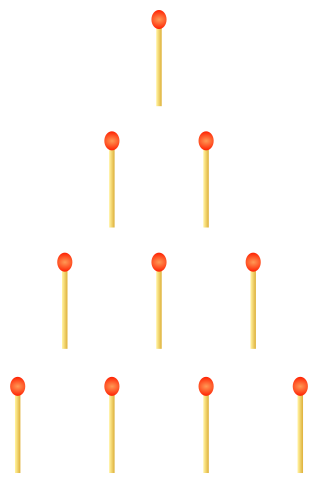
\includegraphics[height=20\baselineskip]{img/Pyramidal_matches.pdf}}\label{img:matches}


\end{frame}
%%%%%%%%%%%%%%%%%%%%%%%%%%%%%%%%%%%%%%%%%%%%%%%%%%%%%%%%%%%%%%%%%%%%%%%%%%%%%%%%%%%%%%%%%%%%

\newcommand{\clou}[2]{\draw[#2] #1 -- +(.4,0) -- +(.2,0) -- +(.2,.5);}
\begin{frame}{Ce qu'il faut retenir du jeu de Nim}

  \begin{block}{L'intérêt majeur de ce jeu est qu'il est sans suspense}
    \begin{itemize}
    \item Celui qui commence perd, car il existe un truc pour gagner à tous
      les coups
    \item \structure{Stratégie gagnante:} Laisser 4, 8, 12 ou 16 clous à
      l'adversaire (un multiple de 4)
    \end{itemize}
  \end{block}

  \begin{block}{Se convaincre de l'efficacité de la stratégie gagnante}
    Prenons le dernier coup comme exemple.
    \begin{itemize}
    \item Si le joueur dont c'est le tour prend 1 clou, son adversaire en prend
      3 et gagne
    \item Si le joueur dont c'est le tour prend 2 clous, son adversaire en
      prend 2 et gagne
    \item Si le joueur dont c'est le tour prend 3 clous, son adversaire en
      prend 1 et gagne 
    \end{itemize}
    Quoi qu'il fasse, le joueur dont c'est le tour a donc perdu si son
    adversaire sait jouer.
  \end{block}

  \begin{center}
    \begin{tabular}{|c|cccc|c|}\hline
      \structure{Situation au dernier tour}
      &
      \multicolumn{4}{c|}{\structure{Évolutions possibles}}&
      \structure{Situation après}
      \\
      &\alert{Joueur 1}&1 clou&2 clous&3 clous&\\\cline{2-5}
      &\structure{Joueur 2}&3 clous&2 clous&1 clou&\\\hline
      Reste 4 clous:
      \begin{tikzpicture}[baseline=\baselineskip]
        \clou{(.5,.6)}{draw=black}
        \clou{(0,0)}{draw=black}
        \clou{(.5,0)}{draw=black}
        \clou{(1,0)}{draw=black}
      \end{tikzpicture}
      &&
      \begin{tikzpicture}[baseline=\baselineskip]
        \clou{(.5,.6)}{draw=blue}
        \clou{(0,0)}{draw=blue}
        \clou{(.5,0)}{draw=blue}
        \clou{(1,0)}{draw=red}
      \end{tikzpicture} &
      \begin{tikzpicture}[baseline=\baselineskip]
        \clou{(.5,.6)}{draw=blue}
        \clou{(0,0)}{draw=blue}
        \clou{(.5,0)}{draw=red}
        \clou{(1,0)}{draw=red}
      \end{tikzpicture} & 
      \begin{tikzpicture}[baseline=\baselineskip]
        \clou{(.5,.6)}{draw=blue}
        \clou{(0,0)}{draw=red}
        \clou{(.5,0)}{draw=red}
        \clou{(1,0)}{draw=red}
      \end{tikzpicture}
      &Joueur 2 gagne
      \\\hline
    \end{tabular}
  \end{center}

  Et le joueur 2 peut faire en sorte qu'on arrive toujours dans cette situation
  depuis le coup précédent:
  \begin{center}
    \begin{tabular}{|c|cccc|c|}\hline
      \structure{Situation au tour d'avant}
      &
      \multicolumn{4}{c|}{\structure{Évolutions possibles}}
      &\structure{Situation après}
      \\
      &\alert{Joueur 1}&1 clou&2 clous&3 clous&\\\cline{2-5}
      &\structure{Joueur 2}&3 clous&2 clous&1 clou&\\\hline
      Reste 8 clous:
      \begin{tikzpicture}[baseline=\baselineskip]
        \clou{(.5,.6)}{draw=black}
        \clou{(0,0)}{draw=black}
        \clou{(.5,0)}{draw=black}
        \clou{(1,0)}{draw=black}
        \clou{(-.5,-.6)}{draw=black}
        \clou{(0,-.6)}{draw=black}
        \clou{(.5,-.6)}{draw=black}
        \clou{(1,-.6)}{draw=black}
      \end{tikzpicture}
      &&
      \begin{tikzpicture}[baseline=\baselineskip]
        \clou{(.5,.6)}{draw=black}
        \clou{(0,0)}{draw=black}
        \clou{(.5,0)}{draw=black}
        \clou{(1,0)}{draw=black}
        \clou{(-.5,-.6)}{draw=blue}
        \clou{(0,-.6)}{draw=blue}
        \clou{(.5,-.6)}{draw=blue}
        \clou{(1,-.6)}{draw=red}
      \end{tikzpicture} &
      \begin{tikzpicture}[baseline=\baselineskip]
        \clou{(.5,.6)}{draw=black}
        \clou{(0,0)}{draw=black}
        \clou{(.5,0)}{draw=black}
        \clou{(1,0)}{draw=black}
        \clou{(-.5,-.6)}{draw=blue}
        \clou{(0,-.6)}{draw=blue}
        \clou{(.5,-.6)}{draw=red}
        \clou{(1,-.6)}{draw=red}
      \end{tikzpicture} & 
      \begin{tikzpicture}[baseline=\baselineskip]
        \clou{(.5,.6)}{draw=black}
        \clou{(0,0)}{draw=black}
        \clou{(.5,0)}{draw=black}
        \clou{(1,0)}{draw=black}
        \clou{(-.5,-.6)}{draw=blue}
        \clou{(0,-.6)}{draw=red}
        \clou{(.5,-.6)}{draw=red}
        \clou{(1,-.6)}{draw=red}
      \end{tikzpicture}
      &Reste 4 clous
      \\\hline
    \end{tabular}
  \end{center}
  Et ainsi de suite
  

  \begin{block}{Le rapport avec l'informatique}
    \begin{itemize}
    \item Passer de la situation initiale à la situation finale à coup sûr demande d'avoir
      une \textit{stratégie gagnante}
    \item C'est un \alert{\textbf{algorithme}} en informatique, une recette de
      cuisine ou un manuel de montage de meubles
    \item Pour se faire obéir du tas de fils, l'informaticien cherche
      l'algorithme pour résoudre le problème,\\
      puis il écrit le \alert{\textbf{programme}} (traduction de l'algorithme
      dans un langage informatique)
    \end{itemize}
  \end{block}
\end{frame}
%%%%%%%%%%%%%%%%%%%%%%%%%%%%%%%%%%%%%%%%%%%%%%%%%%%%%%%%%%%%%%%%%%%%%%%%%%%%%%%%%%%%%%%%%
%%%%%%%%%%%%%%%%%%%%%%%%%%%%%%%%%%%%%%%%%%%%%%%%%%%%%%%%%%%%%%%%%%%%%%%%%%%%%%%%%%%%%%%%%
%%%%%%%%%%%%%%% LE JEU DU CRÊPIER
%%%%%%%%%%%%%%%%%%%%%%%%%%%%%%%%%%%%%%%%%%%%%%%%%%%%%%%%%%%%%%%%%%%%%%%%%%%%%%%%%%%%%%%%%
%%%%%%%%%%%%%%%%%%%%%%%%%%%%%%%%%%%%%%%%%%%%%%%%%%%%%%%%%%%%%%%%%%%%%%%%%%%%%%%%%%%%%%%%%
\begin{frame}{Activité: Le crêpier psycho-rigide}
 
  \begin{block}{Matériel}
    \begin{itemize}
    \item des planchettes en bois de tailles et de couleurs différentes (faces reconnaissables)
    \item éventuellement une pelle à tarte pour retourner les planchettes
    \end{itemize}
  \end{block}
  
  \begin{block}{Règle du jeu}
    \begin{itemize}
    \item Le crêpier doit ranger ses crêpes de la plus grande à la plus petite,
      face colorée vers le haut
    \item il peut retourner une ou plusieurs crêpes à la fois
    \item l'ordre des crêpes ne peut pas être modifié au moment de retouner
      une pile
    \end{itemize}
  \end{block}

%  mettre une illustration ici ?

\end{frame}
%%%%%%%%%%%%%%%%%%%%%%%%%%%%%%%%%%%%%%%%%%%%%%%%%%%%%%%%%%%%%%%%%%%%%%%%%%%%%%%%%%%%%%%%%
\begin{frame}{Ce qu'il faut retenir du  crêpier psycho-rigide}

  \begin{block}{Un algorithme}
    \begin{itemize}
    \item n'a d'intérêt que si on peut l'expliquer
    \item doit être suffisamment simple pour pouvoir l'expliquer à une machine
    \item \alert{\textbf{\og~Diviser pour mieux régner~\fg}} : on essaie
    toujours de décomposer un algorithme en tâches simples
    \end{itemize}
  \end{block}

  \begin{block}{L'algorithme que doit suivre le crêpier est :}
    \begin{itemize}
    \item ramener la plus grande crêpe en haut de la pile
    \item retourner pour que la face brûlée soit vers le haut
    \item retourner la pile de sorte à mettre la plus grande crêpe en bas
    \item réitérer avec la crêpe de taille inférieure
    \end{itemize}
  \end{block}

  \begin{block}{Le rapport avec l'informatique}
    \begin{itemize}
    \item l'informaticien passe son temps à trouver des algorithmes et  à les
    expliquer à la machine
    \item le principe \alert{\textbf{\og~Diviser pour mieux régner~\fg}} est
    fondamental en informatique
    \end{itemize}
  \end{block}
\end{frame}
%%%%%%%%%%%%%%%%%%%%%%%%%%%%%%%%%%%%%%%%%%%%%%%%%%%%%%%%%%%%%%%%%%%%%%%%%%%%%%%%%%%%%%%%%
%%%%%%%%%%%%%%%%%%%%%%%%%%%%%%%%%%%%%%%%%%%%%%%%%%%%%%%%%%%%%%%%%%%%%%%%%%%%%%%%%%%%%%%%%
%%%%%%%%%%%%%%%%%   LES BONSHOMMES
%%%%%%%%%%%%%%%%%%%%%%%%%%%%%%%%%%%%%%%%%%%%%%%%%%%%%%%%%%%%%%%%%%%%%%%%%%%%%%%%%%%%%%%%%
%%%%%%%%%%%%%%%%%%%%%%%%%%%%%%%%%%%%%%%%%%%%%%%%%%%%%%%%%%%%%%%%%%%%%%%%%%%%%%%%%%%%%%%%%
\newcommand{\maisonPair}[5]{  \begin{tikzpicture}
    \node[name=m,shape=regular polygon,regular polygon sides=#3,minimum size=22mm,
          rotate=(360/#3)]{};
    \node[name=b,shape=regular polygon,regular polygon sides=#4,minimum size=14mm,
          rotate=(360/#4)/2]{};
    \foreach \base/\maison in {#5} {
      \draw[shift=(m.corner \base)] 
         node[shape=ellipse,fill=\maison,draw=black,rotate=((360/#3)*(\base-1))+(360/#3/2)] {~~};
    }
    \foreach \bb in {1,...,#4} {
      \draw[shift=(b.corner \bb)] node[name=bb \bb]{};
    }
    \foreach \base/\maison in {#1} {
      \draw[shift=(b.corner \base)] 
         node[name=bb \base,shape=circle,fill=\maison,draw=black,inner sep=.1] 
         {~~~};
%         {\footnotesize\base};
    }
    #2
  \end{tikzpicture}
}
\newcommand{\maisonImpair}[5]{  \begin{tikzpicture}
    \node[name=m,shape=regular polygon,regular polygon sides=#3,minimum size=22mm]{};
    \node[name=b,shape=regular polygon,regular polygon sides=#4,minimum size=14mm]{};
    \foreach \base/\maison in {#5} {
      \draw[shift=(m.corner \base)] 
         node[shape=ellipse,fill=\maison,draw=black,rotate=(360/#3)*(\base-1)] {~~};
    }
    \foreach \base/\maison in {#1} {
      \draw[shift=(b.corner \base)] 
         node[shape=circle,fill=\maison,draw=black,inner sep=.1] {~~~};
    }
    \foreach \bb in {1,...,#4} {\draw[shift=(b.corner \bb)] node[name=bb \bb] {};}
%    \foreach \bb in {1,...,#4} {\draw[shift=(b.corner \bb)] node[name=bb \bb]{\tiny\bb};}%debug the bonshommes names
    #2
  \end{tikzpicture}
}
\newcommand{\maisonQuatre}[2]{\maisonPair{#1}{#2}{4}{12}{1/A,2/B,3/C,4/D}}
\newcommand{\maisonCinq}[2]{\maisonImpair{#1}{#2}{5}{20}{1/A,2/B,3/C,4/D,5/E}}
\newcommand{\maisonSix}[2]{\maisonPair{#1}{#2}{6}{24}{1/A,2/B,3/C,4/D,5/E,6/F}}
\newcommand{\maisonSept}[2]{\maisonImpair{#1}{#2}{7}{28}{1/A,2/B,3/C,4/D,5/E,6/F,7/G}}

\colorlet{A}{green!60}
\colorlet{B}{red!80}
\colorlet{C}{purple!40}
\colorlet{D}{orange!80}
\colorlet{E}{blue!80}
\colorlet{F}{black!10!yellow}
\colorlet{G}{olive}
\colorlet{H}{magenta}
\colorlet{I}{lime}
\colorlet{J}{pink}

%%%%%%%%%%%%%%%%%%%%%%%%%%%%%%%%%%%%%%%%%%%%%%%%%%%%%%%%%%%%%%%%%%%%%%%%%%%%%%%%%%%%%%%
\begin{frame}{Activité: Base-ball multicolor}
  \begin{block}{Matériel nécessaire}
    \begin{itemize}
    \item Plusieurs équipes bien différenciables, chacune composée d'une maison
      et de deux bonshommes\\
      (des legos, des bouts de bois, des caillous, du fil électrique de
      différentes couleurs, ou autres)
      
    \item Il faut 5 équipes au minimum. 7 équipes sont préférables, et on peut
      en utiliser une dizaine
    \end{itemize}
  \end{block}

  \begin{block}{Règles du jeu à quatre équipes}
    \begin{itemize}
    \item \structure{Situation initiale:}~\\
      On place 4 maisons autour du terrain, et on réparti 7 bonshommes au
      hasard dans les maisons\\
     (il manque donc l'un des bonshommes, qui est mis de coté et ne sera
      pas utilisé)
    \item \structure{Coups autorisés:}
      \begin{itemize}\normalsize
      \item On peut déplacer un seul bonhomme à la fois, d'une maison vers une
        maison adjacente\\
        $\leadsto$ il est interdit de traverser le terrain
      \item On ne peut jamais avoir plus de 2 bonshommes par maison\\
        $\leadsto$ on ne peut bouger que d'une maison adjacente vers la maison
        où il y a un trou
      \end{itemize}
    \item  \structure{Situation finale:}
      L'objectif est de ramener tous les bonshommes dans la maison de leur couleur.
    \end{itemize}
  \end{block}

  \vspace{-\baselineskip}
  \begin{columns}
    \begin{column}{.17\linewidth}\center
      \maisonQuatre{2/B,3/A, 5/D, 8/B,9/C, 11/D,12/A} {}

      \structure{Situation initiale}      
    \end{column}
    \begin{column}{.17\linewidth}\center
      \maisonQuatre{2/B,3/A, 5/D, 8/B,9/C, 11/D,12/A}
                   { 
                     \draw[->,ultra thick,draw=black!10!green] (bb 2) -> (bb 6);
                     \draw[->,ultra thick,draw=black!10!green] (bb 3) -> (bb 6);
                     \draw[->,ultra thick,draw=black!10!green] (bb 9) -> (bb 6);
                     \draw[->,ultra thick,draw=black!10!green] (bb 8) -> (bb 6);}

      \structure{Coups autorisés}      
    \end{column}
    \begin{column}{.17\linewidth}\center
      \maisonQuatre{2/B,3/A, 5/D, 8/B,9/C, 11/D,12/A}
                   { \draw[->,ultra thick,draw=red] (bb 11) -> (bb 6);
                     \draw[->,ultra thick,draw=red] (bb 12) -> (bb 6);
                     \draw[->,ultra thick,draw=red] (bb 12) -> (bb 2);
                     \draw[->,ultra thick,draw=red] (bb 2) -> (bb 12);
                     \draw[->,ultra thick,draw=red] (bb 5) -> (bb 3);
                     \draw[->,ultra thick,draw=red] (bb 5) 
                        .. controls (0pt,0pt) .. (bb 8);
                     \draw[->,ultra thick,draw=red] (bb 11) -> (bb 9);
                     \draw[->,ultra thick,draw=red] (bb 9) -> (bb 11);
                   }

      \structure{Coups interdits}      
    \end{column}
    \begin{column}{.17\linewidth}\center
      \maisonQuatre{2/A,3/A, 5/B,6/B, 8/C,9/C, 11/D}{}

      \structure{Situation finale}      
    \end{column}
  \end{columns}

  \bigskip
  \begin{block}{Objectif de l'activité}
    \begin{itemize}
    \item Le plus important n'est pas  de ramener les bonshommes dans leurs
      maisons
    \item L'objectif est d'expliquer comment on fait. On cherche donc
      l'algorithme correspondant
    \item Si on veut utiliser plus de couleurs, c'est possible.
    \end{itemize}
  \end{block}

  \centerline{
    \maisonCinq{1/A,2/A, 5/B,6/B, 9/C,10/C, 13/D,14/D, 17/E}{}  
    \maisonSix{2/A,4/A,  6/B,8/B, 10/C,12/C, 14/D,16/D, 18/E,20/E, 22/F}{}  
    \maisonSept{1/A,2/A, 5/B,6/B, 9/C,10/C, 13/D,14/D, 17/E,18/E, 21/F,22/F, 25/G}{}  
    \maisonPair{2/A,4/A, 6/B,8/B, 10/C,12/C, 14/D,16/D, 18/E,20/E, 22/F,24/F,
      26/G,28/G, 30/H}{}{8}{32}
               {1/A,2/B,3/C,4/D,5/E,6/F,7/G,8/H}
    % Neuf maisons
    \maisonImpair{1/A,2/A, 5/B,6/B, 9/C,10/C, 13/D,14/D, 17/E,18/E,
                  21/F,22/F, 25/G,26/G, 29/H,30/H,  33/I}{}{9}{36}
               {1/A,2/B,3/C,4/D,5/E,6/F,7/G,8/H,9/I}
    % Dix maisons
    \maisonPair{2/A,4/A, 6/B,8/B, 10/C,12/C, 14/D,16/D, 18/E,20/E, 22/F,24/F,
      26/G,28/G, 30/H,32/H, 34/I,36/I, 38/J}{}{10}{40}
               {1/A,2/B,3/C,4/D,5/E,6/F,7/G,8/H,9/I,10/J}
  }

  
\end{frame}
%%%%%%%%%%%%%%%%%%%%%%%%%%%%%%%%%%%%%%%%%%%%%%%%%%%%%%%%%%%%%%%%%%%%%%%%%%%%%%%%%%%%%%%%%
\newcommand{\flecherond}[1]{
  \draw[ultra thick] (0,0) circle (3mm);
  \draw[ultra thick,rotate=#1*72] (3mm,0) -- +(-.15,-.08);
  \draw[ultra thick,rotate=#1*72] (3mm,0) -- +(.08,-.15);
  \draw[fill=white,draw=white,rotate=#1*72] (3mm,2.5pt) circle (2pt);
}
\begin{frame}<0>{Un premier algorithme pour le base-ball multicolor}
  \begin{block}{L'algorithme}
    \begin{itemize}
    \item On ne s'autorise qu'à tourner dans un seul sens.
    \item On n'a plus 4 coups possibles, mais deux seulement (car 2 bonshommes
      tourneraient à l'envers)
    \item Entre ces deux bonshommes, je déplace celui dont la destination est la
      plus lointaine
    \end{itemize}
  \end{block}


  \begin{block}{Exemple d'exécution}
    \begin{columns}
      % J'avais une case de trop...
      % \begin{column}{.15\linewidth}\center
      %   \maisonCinq{1/D,2/B, 5/A,6/C, 9/E,10/D, 13/A,14/C, 17/B}{\flecherond{0}}\\
      %   {\small $4>2\Rightarrow$ violet}        
      % \end{column}

      \begin{column}{.15\linewidth}\center
        \maisonCinq{1/D,2/B, 5/A,6/C, 9/E,10/D, 13/A, 17/B,18/C}{\flecherond{4}}\\
        {\small $2>1\Rightarrow$ bleu}        
      \end{column}

      \begin{column}{.15\linewidth}\center
        \maisonCinq{1/D,2/B, 5/A,6/C, 10/D, 13/A,14/E, 17/B,18/C}{\flecherond{3}}\\
        {\small $4>1\Rightarrow$ vert}        
      \end{column}

      \begin{column}{.15\linewidth}\center
        \maisonCinq{1/D,2/B, 6/C, 9/A,10/D, 13/A,14/E, 17/B,18/C}{\flecherond{2}}\\
        {\small $3>1\Rightarrow$ orange}        
      \end{column}

      \begin{column}{.15\linewidth}\center
        \maisonCinq{2/B, 5/D,6/C, 9/A,10/D, 13/A,14/E, 17/B,18/C}{\flecherond{1}}\\
        {\small $3>2\Rightarrow$ violet}        
      \end{column}
      \begin{column}{.15\linewidth}\center
        \maisonCinq{1/C,2/B, 5/D,6/C, 9/A,10/D, 13/A,14/E, 17/B}{\flecherond{0}}\\
        {\small $2>1\Rightarrow$ vert}        
      \end{column}
    \end{columns}
    %%%%%%%%%%%%%
    \begin{columns}
      \begin{column}{.15\linewidth}\center
        \maisonCinq{1/C,2/B, 5/D,6/C, 9/A,10/D, 14/E, 17/B,18/A}{\flecherond{4}}\\
        {\small $2>1\Rightarrow$ vert}        
      \end{column}

      \begin{column}{.15\linewidth}\center
        \maisonCinq{1/C,2/B, 5/D,6/C, 10/D, 13/A,14/E, 17/B,18/A}{\flecherond{3}}\\
         {\small $2>1\Rightarrow$ orange}        
      \end{column}

      \begin{column}{.15\linewidth}\center
        \maisonCinq{1/C,2/B, 6/C, 9/D,10/D, 13/A,14/E, 17/B,18/A}{\flecherond{2}}\\
         {\small $2>1\Rightarrow$ violet}        
      \end{column}

      \begin{column}{.15\linewidth}\center
        \maisonCinq{2/B, 5/C,6/C, 9/D,10/D, 13/A,14/E, 17/B,18/A}{\flecherond{1}}\\
         {\small $2>1\Rightarrow$ rouge}        
      \end{column}
      \begin{column}{.15\linewidth}\center
        \maisonCinq{1/B,2/B, 5/C,6/C, 9/D,10/D, 13/A,14/E, 18/A}{\flecherond{0}}\\
         {\small $2>1\Rightarrow$ vert}        
      \end{column}
    \end{columns}
    %%%%%%%%%%%%%
    \begin{columns}
      \begin{column}{.15\linewidth}\center
        \maisonCinq{1/B,2/B, 5/C,6/C, 9/D,10/D, 14/E, 17/A,18/A}{\flecherond{4}}\\
         {\small $1=1\Rightarrow$ orange}        
      \end{column}

      \begin{column}{.15\linewidth}\center
        \maisonCinq{1/B,2/B, 5/C,6/C, 10/D, 13/D,14/E, 17/A,18/A}{\flecherond{3}}\\
         {\small $1=1\Rightarrow$ violet}        
      \end{column}

      \begin{column}{.15\linewidth}\center
        \maisonCinq{1/B,2/B, 6/C, 9/C,10/D, 13/D,14/E, 17/A,18/A}{\flecherond{2}}\\
         {\small $1=1\Rightarrow$ rouge}        
      \end{column}

      \begin{column}{.15\linewidth}\center
        \maisonCinq{2/B, 5/B,6/C, 9/C,10/D, 13/D,14/E, 17/A,18/A}{\flecherond{1}}\\
         {\small $1=1\Rightarrow$ vert}        
      \end{column}

      \begin{column}{.15\linewidth}\center
        \maisonCinq{1/A,2/B, 5/B,6/C, 9/C,10/D, 13/D,14/E, 18/A}{\flecherond{0}}\\
         {\small $1>0\Rightarrow$ bleu}        
      \end{column}
    \end{columns}
    %%%%%%%%%%%%%
    \begin{columns}[t]
      \begin{column}{.15\linewidth}\center
        \maisonCinq{1/A,2/B, 5/B,6/C, 9/C,10/D, 13/D, 17/E,18/A}{\flecherond{4}}\\
         {\small $1>0\Rightarrow$ orange}
      \end{column}

      \begin{column}{.15\linewidth}\center
        \maisonCinq{1/A,2/B, 5/B,6/C, 9/C, 13/D,14/D, 17/E,18/A}{\flecherond{3}}\\
         {\small $1>0\Rightarrow$ violet}
      \end{column}

      \begin{column}{.15\linewidth}\center
        \maisonCinq{1/A,2/B, 5/B, 9/C,10/C, 13/D,14/D, 17/E,18/A}{\flecherond{2}}\\
         {\small $1>0\Rightarrow$ rouge}
      \end{column}

      \begin{column}{.15\linewidth}\center
        \maisonCinq{1/A, 5/B,6/B, 9/C,10/C, 13/D,14/D, 17/E,18/A}{\flecherond{1}}\\
         {\small $1>0\Rightarrow$ vert}
      \end{column}

      \begin{column}{.15\linewidth}\center
        \maisonCinq{1/A,2/A, 5/B,6/B, 9/C,10/C, 13/D,14/D, 17/E}{\flecherond{0}}\\
         {\small $1>0\Rightarrow$ vert}

         \alert{Gagné!}
      \end{column}
    \end{columns}
  \end{block}
\end{frame}
%%%%%%%%%%%%%%%%%%%%%%%%%%%%%%%%%%%%%%%%%%%%%%%%%%%%%%%%%%%%%%%%%%%%%%%%%%%%%%%%%%%%%%%%%
\begin{frame}{Étude du premier algorithme pour le base-ball multicolor}
  \begin{block}{Cet algorithme est bel et bon}
    \begin{itemize}
    \item Il est très simple: on pourrait l'expliquer à un ordinateur
    \item Il est relativement rapide: 20 coups pour 9 bonshommes, ce n'est pas
      si mal
    \item Seul problème: cet algorithme est faux: dans certains cas, il ne
      termine jamais\ldots
    \end{itemize}
  \end{block}

  \begin{block}{Exemple d'exécution incorrecte}
    \begin{columns}[t]
      \begin{column}{.15\linewidth}\center
        \maisonCinq{1/A,2/D, 5/B,6/B, 9/C,10/C, 13/A,14/D, 17/E}{\flecherond{0}}\\
         {\small $2>0\Rightarrow$ vert}
      \end{column}
    \end{columns}
  \end{block}
\end{frame}

%%%%%%%%%%%%%%%%%%%%%%%%%%%%%%%%%%%%%%%%%%%%%%%%%%%%%%%%%%%%%%%%%%%%%%%%%%%%%%%%%%%%%%%%%
%%%%%%%%%%%%%%%%%%%%%%%%%%%%%%%%%%%%%%%%%%%%%%%%%%%%%%%%%%%%%%%%%%%%%%%%%%%%%%%%%%%%%%%%%
%%%%%%%%%%%%%%%%%%%%%%%%%%%%%%%%%%%%%%%%%%%%%%%%%%%%%%%%%%%%%%%%%%%%%%%%%%%%%%%%%%%%%%%%%
%%%%%%%%%%%%%%%%%%%%%%%%%%%%%%%%%%%%%%%%%%%%%%%%%%%%%%%%%%%%%%%%%%%%%%%%%%%%%%%%%%%%%%%%%
\begin{frame}{Le coin de l'animateur\\[-5pt]
  {\large Trucs et astuces pour simplifier la présentation de la séance}}
  \begin{block}{Remarques générales}
    \begin{itemize}
    \item Il faut vous approprier les activités. N'hésitez pas à ne pas suivre
      les consignes à la lettre, l'important est que cela vous plaise.
    \end{itemize}
  \end{block}
  \begin{block}{À propos du mot d'introduction}
    \begin{itemize}
    \item On peut faire cette présentation soit au début, soit juste après
      l'activité sur le jeu de Nim. Commencer directement par un petit jeu
      permet d'éviter que les participants ne décrochent avant même qu'on ne commence.
    \end{itemize}
  \end{block}
  \begin{block}{À propos du jeu de Nim}
    \begin{itemize}
    \item L'objectif de cette activité est simplement d'introduire la notion d'algorithme
    \item On propose le jeu avec le participant, mais sans dire trop vite qu'on
      a un truc. S'il y a plusieurs participants, on jouera avec plusieurs
      personnes, pour laisser sa chance à chacun. On peut faire une sorte de
      petit tournois.
    \item Il faut bien sûr laisser commencer le participant pour gagner à coup
      sûr. S'il insiste pour ne pas commencer, on peut le faire (et rattraper
      la stratégie gagnante à la première erreur du participant)
    \item On n'introduit l'existence du truc pour gagner que plus tard, quand
      on gagne à plate couture
    \item Si on perd, c'est à dire si on n'a pas réussi à appliquer la
      stratégie gagnante, il faut proposer un match en 3 (ou en 5 en cas de
      coup dur ;)
    \item Attention, il faut parvenir à compter les clous discrètement\ldots
    \item On peut amener le participant à découvrir la stratégie gagnante en
      groupant les clous par paquets de 4 au lieu de la disposition pyramidale.
    \item Si l'un des participants connaît déjà la stratégie gagnante du jeu,
      il peut remplacer l'animateur dans une partie avec d'autres participants
    \end{itemize}    
  \end{block}
\end{frame}

\begin{frame}{Le coin de l'animateur\\[-5pt]
  {\large Trucs et astuces pour simplifier la présentation de la séance}}
  \begin{block}{À propos du jeu du crêpier psycho-rigide}
    \begin{itemize}
    \item L'objectif de cette activité est de trouver un algorithme et de
    l'expliquer 
    \item On propose au participant de d'abord tenter de le résoudre
    intuitivement, sans réfléchir
    \item Si le participant bloque, on peut lui donner un conseil : \og~Une
    bonne première étape est de se débrouiller pour mettre la grande en bas~\fg
    \item Si le participant bloque toujours, on peut lui donner un second
    conseil : \og~où est-ce que la grande devrait être pour pouvoir la mettre en
    bas ? ~\fg puis le guider pour l'étape suivante.
    \item On essaie ensuite de faire expliquer l'algorithme par le participant.
    On gagne à ce que ce soit le participant et non l'animateur qui explique aux
    autres, avec ses propres mots.
    \end{itemize}    
  \end{block}
%\url{http://interstices.info/jcms/n_52318/genese-dun-algorithme?hlText=cr\%C3\%A8pes}

\end{frame}
\end{document}
